% Slutsky Decomposition: Dynamic Response to Income Shocks
% Shows how TN (fixed-dollar) and FL (tuition-scaling) respond differently

\begin{figure}[t]
\centering
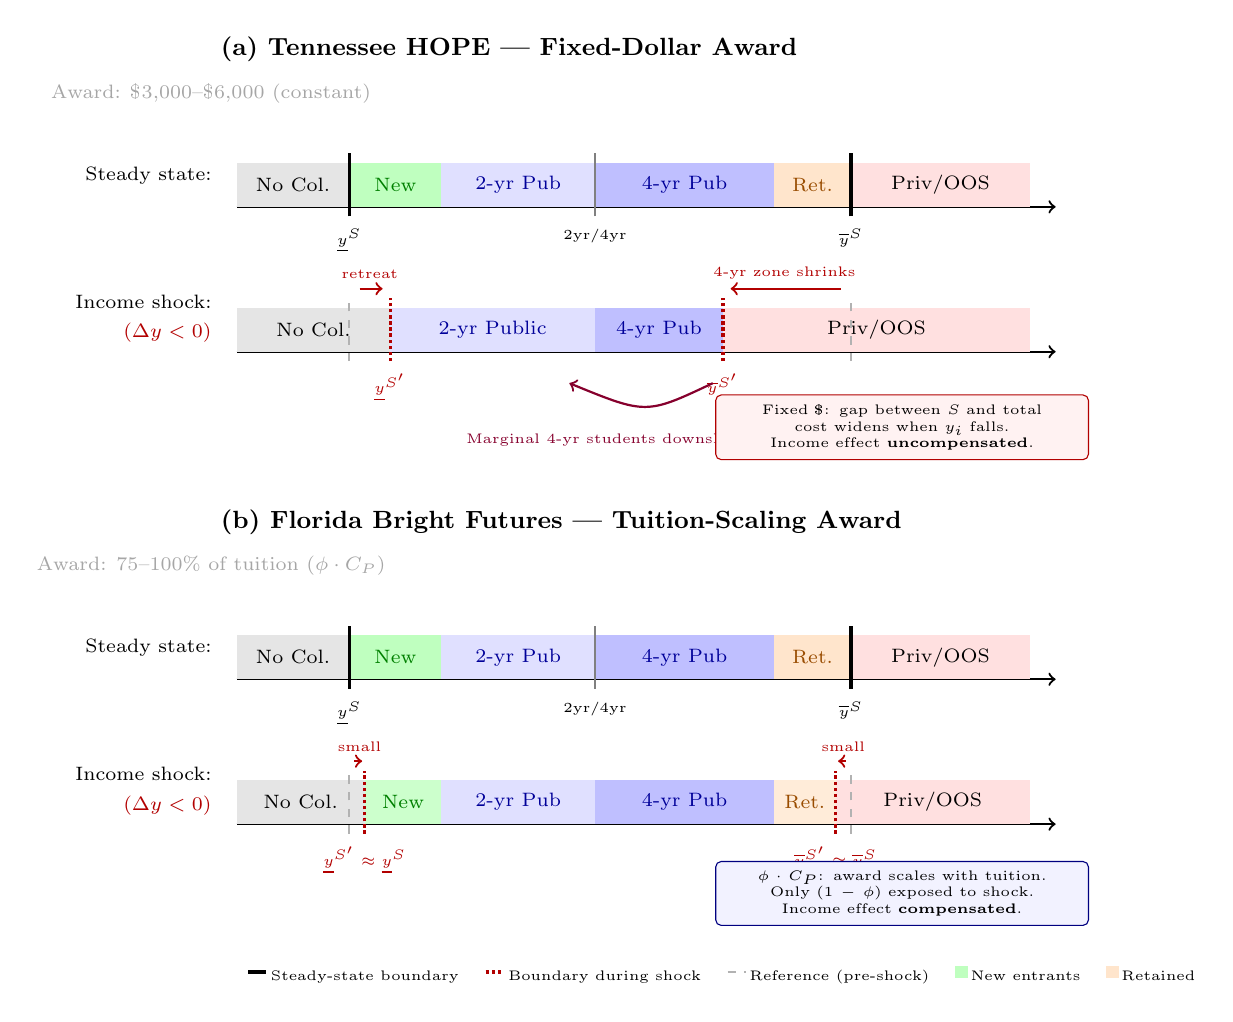
\begin{tikzpicture}[
  x=0.65cm, y=0.8cm,
  region/.style={minimum height=0.7cm, text=black, font=\scriptsize},
  boundary/.style={thick, dashed, gray!60},
  newboundary/.style={very thick, black},
  shockboundary/.style={very thick, red!70!black, densely dotted},
  panellabel/.style={font=\small\bfseries, anchor=west},
  legendbox/.style={font=\tiny, anchor=west},
  ann/.style={font=\scriptsize},
]

% ============================================================
% Panel A: Tennessee HOPE — Fixed-Dollar ($S)
% Before and after income shock
% ============================================================
\node[panellabel] at (-0.5, 14.5)
  {(a) Tennessee HOPE --- Fixed-Dollar Award};
\node[ann, gray!70] at (-0.5, 13.8)
  {Award: \$3{,}000--\$6{,}000 (constant)};

% --- Top bar: Steady state (post-HOPE, no shock) ---
\node[ann, anchor=east] at (-0.3, 12.5) {Steady state:};

\draw[thick, ->] (0, 12.0) -- (16, 12.0);

% Regions: steady state
\fill[gray!20] (0, 12.0) rectangle (2.2, 12.7);
\fill[green!25] (2.2, 12.0) rectangle (4, 12.7);
\fill[blue!12] (4, 12.0) rectangle (7, 12.7);
\fill[blue!25] (7, 12.0) rectangle (10.5, 12.7);
\fill[orange!20] (10.5, 12.0) rectangle (12, 12.7);
\fill[red!12] (12, 12.0) rectangle (15.5, 12.7);

\node[region] at (1.1, 12.35) {No Col.};
\node[region, green!50!black] at (3.1, 12.35) {New};
\node[region, blue!60!black] at (5.5, 12.35) {2-yr Pub};
\node[region, blue!60!black] at (8.75, 12.35) {4-yr Pub};
\node[region, orange!60!black] at (11.25, 12.35) {Ret.};
\node[region] at (13.75, 12.35) {Priv/OOS};

% Boundaries
\draw[newboundary] (2.2, 11.85) -- (2.2, 12.85);
\draw[gray, thin] (7, 11.85) -- (7, 12.85);
\draw[newboundary] (12, 11.85) -- (12, 12.85);
\node[font=\tiny, below] at (2.2, 11.8) {$\underline{y}^S$};
\node[font=\tiny, below] at (7, 11.8) {2yr/4yr};
\node[font=\tiny, below] at (12, 11.8) {$\overline{y}^S$};

% --- Bottom bar: During income shock ---
\node[ann, anchor=east] at (-0.3, 10.5) {Income shock:};
\node[ann, anchor=east, red!70!black] at (-0.3, 10.0) {$(\Delta y < 0)$};

\draw[thick, ->] (0, 9.7) -- (16, 9.7);

% Regions: during shock — boundaries shift BACK
\fill[gray!20] (0, 9.7) rectangle (3.0, 10.4);
\fill[blue!12] (3.0, 9.7) rectangle (7, 10.4);
\fill[blue!25] (7, 9.7) rectangle (9.5, 10.4);
\fill[red!12] (9.5, 9.7) rectangle (15.5, 10.4);

\node[region] at (1.5, 10.05) {No Col.};
\node[region, blue!60!black] at (5.0, 10.05) {2-yr Public};
\node[region, blue!60!black] at (8.25, 10.05) {4-yr Pub};
\node[region] at (12.5, 10.05) {Priv/OOS};

% Shock boundaries (dotted red)
\draw[shockboundary] (3.0, 9.55) -- (3.0, 10.55);
\draw[shockboundary] (9.5, 9.55) -- (9.5, 10.55);
\node[font=\tiny, red!70!black, below] at (3.0, 9.5)
  {$\underline{y}^{S'}$};
\node[font=\tiny, red!70!black, below] at (9.5, 9.5)
  {$\overline{y}^{S'}$};

% Original boundaries (dashed gray for reference)
\draw[boundary] (2.2, 9.55) -- (2.2, 10.55);
\draw[boundary] (12, 9.55) -- (12, 10.55);

% Arrows showing retreat
\draw[thick, ->, red!70!black] (2.4, 10.7) -- (2.85, 10.7);
\node[ann, red!70!black, above] at (2.6, 10.7) {\tiny retreat};

\draw[thick, <-, red!70!black] (9.65, 10.7) -- (11.8, 10.7);
\node[ann, red!70!black, above] at (10.7, 10.7) {\tiny 4-yr zone shrinks};

% Annotation: marginal students
\draw[thick, ->, purple!70!black] (9.3, 9.2) .. controls (8, 8.7)
  .. (6.5, 9.2);
\node[font=\tiny, purple!70!black, below] at (7.8, 8.55)
  {Marginal 4-yr students downshift to 2-yr};

% Box annotation
\node[draw=red!70!black, rounded corners=2pt, fill=red!5,
  font=\tiny, text width=4.5cm, align=center] at (13, 8.5)
  {Fixed \$: gap between $S$ and total\\
   cost widens when $y_i$ falls.\\
   Income effect \textbf{uncompensated}.};


% ============================================================
% Panel B: Florida Bright Futures — Percentage-Based (φ·C_P)
% ============================================================
\node[panellabel] at (-0.5, 7.0)
  {(b) Florida Bright Futures --- Tuition-Scaling Award};
\node[ann, gray!70] at (-0.5, 6.3)
  {Award: 75--100\% of tuition ($\phi \cdot C_P$)};

% --- Top bar: Steady state ---
\node[ann, anchor=east] at (-0.3, 5.0) {Steady state:};

\draw[thick, ->] (0, 4.5) -- (16, 4.5);

\fill[gray!20] (0, 4.5) rectangle (2.2, 5.2);
\fill[green!25] (2.2, 4.5) rectangle (4, 5.2);
\fill[blue!12] (4, 4.5) rectangle (7, 5.2);
\fill[blue!25] (7, 4.5) rectangle (10.5, 5.2);
\fill[orange!20] (10.5, 4.5) rectangle (12, 5.2);
\fill[red!12] (12, 4.5) rectangle (15.5, 5.2);

\node[region] at (1.1, 4.85) {No Col.};
\node[region, green!50!black] at (3.1, 4.85) {New};
\node[region, blue!60!black] at (5.5, 4.85) {2-yr Pub};
\node[region, blue!60!black] at (8.75, 4.85) {4-yr Pub};
\node[region, orange!60!black] at (11.25, 4.85) {Ret.};
\node[region] at (13.75, 4.85) {Priv/OOS};

\draw[newboundary] (2.2, 4.35) -- (2.2, 5.35);
\draw[gray, thin] (7, 4.35) -- (7, 5.35);
\draw[newboundary] (12, 4.35) -- (12, 5.35);
\node[font=\tiny, below] at (2.2, 4.3) {$\underline{y}^S$};
\node[font=\tiny, below] at (7, 4.3) {2yr/4yr};
\node[font=\tiny, below] at (12, 4.3) {$\overline{y}^S$};

% --- Bottom bar: During income shock — boundaries barely move ---
\node[ann, anchor=east] at (-0.3, 3.0) {Income shock:};
\node[ann, anchor=east, red!70!black] at (-0.3, 2.5) {$(\Delta y < 0)$};

\draw[thick, ->] (0, 2.2) -- (16, 2.2);

% Nearly identical to steady state
\fill[gray!20] (0, 2.2) rectangle (2.5, 2.9);
\fill[green!20] (2.5, 2.2) rectangle (4, 2.9);
\fill[blue!12] (4, 2.2) rectangle (7, 2.9);
\fill[blue!25] (7, 2.2) rectangle (10.5, 2.9);
\fill[orange!15] (10.5, 2.2) rectangle (11.7, 2.9);
\fill[red!12] (11.7, 2.2) rectangle (15.5, 2.9);

\node[region] at (1.25, 2.55) {No Col.};
\node[region, green!50!black] at (3.25, 2.55) {New};
\node[region, blue!60!black] at (5.5, 2.55) {2-yr Pub};
\node[region, blue!60!black] at (8.75, 2.55) {4-yr Pub};
\node[region, orange!60!black] at (11.1, 2.55) {Ret.};
\node[region] at (13.6, 2.55) {Priv/OOS};

% Shock boundaries (barely moved)
\draw[shockboundary] (2.5, 2.05) -- (2.5, 3.05);
\draw[shockboundary] (11.7, 2.05) -- (11.7, 3.05);

% Original boundaries for reference
\draw[boundary] (2.2, 2.05) -- (2.2, 3.05);
\draw[boundary] (12, 2.05) -- (12, 3.05);

\node[font=\tiny, red!70!black, below] at (2.5, 2.0)
  {$\underline{y}^{S'} \approx \underline{y}^S$};
\node[font=\tiny, red!70!black, below] at (11.7, 2.0)
  {$\overline{y}^{S'} \approx \overline{y}^S$};

% Small arrows showing minimal retreat
\draw[thick, ->, red!70!black] (2.3, 3.2) -- (2.45, 3.2);
\node[ann, red!70!black, above] at (2.4, 3.2) {\tiny small};

\draw[thick, <-, red!70!black] (11.75, 3.2) -- (11.9, 3.2);
\node[ann, red!70!black, above] at (11.85, 3.2) {\tiny small};

% Box annotation
\node[draw=blue!50!black, rounded corners=2pt, fill=blue!5,
  font=\tiny, text width=4.5cm, align=center] at (13, 1.1)
  {$\phi \cdot C_P$: award scales with tuition.\\
   Only $(1-\phi)$ exposed to shock.\\
   Income effect \textbf{compensated}.};


% ============================================================
% Legend
% ============================================================
\node[legendbox] at (0, -0.2) {%
  \tikz[baseline=-0.5ex]{\draw[very thick, black] (0,0.09) -- (0.35,0.09);}\,Steady-state boundary \quad
  \tikz[baseline=-0.5ex]{\draw[very thick, red!70!black, densely dotted] (0,0.09) -- (0.35,0.09);}\,Boundary during shock \quad
  \tikz[baseline=-0.5ex]{\draw[thick, dashed, gray!60] (0,0.09) -- (0.35,0.09);}\,Reference (pre-shock) \quad
  \tikz[baseline=-0.5ex]{\fill[green!25] (0,0) rectangle (0.25,0.18);}\,New entrants \quad
  \tikz[baseline=-0.5ex]{\fill[orange!20] (0,0) rectangle (0.25,0.18);}\,Retained
};

\end{tikzpicture}

\caption{Slutsky Decomposition: How Award Structure Determines
  Resilience to Income Shocks}
\label{fig:decomposition}

\vspace{1mm}
\begin{minipage}{0.92\textwidth}
  \footnotesize
  \textit{Notes:} Each panel shows the steady-state sorting (top bar)
  and the response to a negative income shock (bottom bar). Panel~(a):
  Tennessee HOPE pays a fixed dollar amount (\$3,000--\$6,000). When
  income falls, the gap between the award and total cost of attendance
  widens. Both boundaries retreat substantially: some new entrants at
  the access margin drop out, and marginal four-year students (created
  by HOPE) downshift to two-year colleges. The income effect is
  uncompensated. Panel~(b): Florida Bright Futures covers a fixed
  percentage of tuition (75--100\%). When income falls, the award
  scales with tuition costs, so the gap between scholarship and cost
  barely changes. Boundaries shift minimally. The income effect is
  compensated. Both programs produce progressive sorting in steady
  state (the substitution effect); only the percentage-based program
  sustains it during downturns.
\end{minipage}
\end{figure}
